\let\negmedspace\undefined
\let\negthickspace\undefined
\documentclass[journal]{IEEEtran}
\usepackage[a5paper, margin=10mm, onecolumn]{geometry}
%\usepackage{lmodern} % Ensure lmodern is loaded for pdflatex
\usepackage{tfrupee} % Include tfrupee package

\setlength{\headheight}{1cm} % Set the height of the header box
\setlength{\headsep}{0mm}     % Set the distance between the header box and the top of the text

\usepackage{gvv-book}
\usepackage{gvv}
\usepackage{cite}
\usepackage{amsmath,amssymb,amsfonts,amsthm}
\usepackage{algorithmic}
\usepackage{graphicx}
\usepackage{textcomp}
\usepackage{xcolor}
\usepackage{txfonts}
\usepackage{listings}
\usepackage{enumitem}
\usepackage{mathtools}
\usepackage{gensymb}
\usepackage{comment}
\usepackage[breaklinks=true]{hyperref}
\usepackage{tkz-euclide}
\usepackage{listings}
% \usepackage{gvv}
\def\inputGnumericTable{}
\usepackage[latin1]{inputenc}
\usepackage{color}
\usepackage{array}
\usepackage{longtable}
\usepackage{calc}
\usepackage{multirow}
\usepackage{hhline}
\usepackage{ifthen}
\usepackage{lscape}
\begin{document}

\bibliographystyle{IEEEtran}

\title{9.4.36}
\author{EE25BTECH11023 - Venkata Sai}
% \maketitle
% \newpage
% \bigskip
\maketitle
\renewcommand{\thefigure}{\theenumi}
\renewcommand{\thetable}{\theenumi}
\setlength{\intextsep}{10pt} % Space between text and floats

\numberwithin{align}{enumi}
\numberwithin{figure}{enumi}
\renewcommand{\thetable}{\theenumi}
\vspace{-2em}
\textbf{Question:}  \\
The sum of the reciprocals of Ram's ages, (in years) 3 years ago and 5 years from
now is $\frac{1}{3}$ . Find his present age\\
\textbf{Solution:}  \\
 The input parameters are available in Table 1.\\
\begin{tabular}{|c|c|}
\hline
\textbf{Name} & \textbf{Value} \\ \hline
$\vec{A}$ & $\myvec{2 & 1 \\0 & 3}$ \\ \hline
\end{tabular}

Given sum of reciprocal of Ram's ages 3 years ago and 5 years from
now is $\frac{1}{3}$
\begin{align}
\frac{1}{x-3}+\frac{1}{x+5}=\frac{1}{3} \\
\frac{\brak{x+5}+\brak{x-3}}{\brak{x-3}\brak{x+5}}=\frac{1}{3} \\
\frac{2x+2}{x^2+5x-3x-15}=\frac{1}{3}\\
\frac{2x+2}{x^2+2x-15}=\frac{1}{3}\\
\brak{2x+2}=x^2+2x-15\\
6x+6=x^2+2x-15 \\
x^2+2x-15-6x-6=0 \\
x^2-4x-21=0 \\
\implies y=x^2-4x-21 \\
\implies x^2-4x-y-21=0\\
x^2+2(-2x-\frac{1}{2}y)-21=0
  \end{align}
  which can be expressed as the conic
  \begin{align}
       \vec{x}^\top\vec{V}\vec{x} + 2\vec{u}^\top\vec{x} + f &= 0 \\
       \vec{V}=\myvec{1 & 0 \\ 0&0},\vec{u}=\myvec{-2\\-\frac{1}{2}},f=-21
  \end{align}
  To find the roots of (9), we find the points of intersection of the conic with
the x-axis
\begin{align}
\vec{x}=\vec{h}+k\vec{m}\\
\vec{h}=\myvec{0\\0},\vec{m}=\myvec{1\\0}
\end{align}
\begin{align}
\kappa_i= \frac{1}{\vec{m}^\top \vec{V}\vec{m}}\brak{
       -\,\vec{m}^\top\brak{\vec{V}\vec{h}+\vec{u}}
       \;\pm\;
       \sqrt{ \cbrak{\vec{m}^\top(\vec{V}\vec{h}+\vec{u})}^2
       - g(\vec{h})\,\big(\vec{m}^\top \vec{V}\vec{m}\big)}
     }\\
\end{align}
where
\begin{align}
g\brak{\vec{h}} &= \vec{h}^\top\vec{V}\vec{h}+2\vec{u}^\top\vec{h}+f \\
g\brak{\vec{h}} &= \myvec{0\\0}^\top\myvec{1&0\\0&0}\myvec{0\\0}+2\myvec{-2\\-\frac{1}{2}}^\top\myvec{0\\0}-21 \\
g\brak{\vec{h}} &= \myvec{0&0}\myvec{1&0\\0&0}\myvec{0\\0}+2\myvec{-2&-\frac{1}{2}}\myvec{0\\0}-21 \\
g\brak{\vec{h}} &= \myvec{0&0}\myvec{0\\0}+2\brak{0}-21 \\
g\brak{\vec{h}} &= 0+0-21=-21
\end{align}
     \begin{align}
     \vec{m}^\top \vec{V}\vec{m}=\myvec{1\\0}^\top\myvec{1&0\\0&0}\myvec{1\\0}=\myvec{1&0}\myvec{1&0\\0&0}\myvec{1\\0}=\myvec{1&0}\myvec{1\\0}=1
     \end{align}
     \begin{align}
    \vec{m}^\top\brak{\vec{V}\vec{h}+\vec{u}}
    = \myvec{1\\0}^\top\brak{\myvec{1&0\\0&0}\myvec{0\\0}+\myvec{-2\\-\frac{1}{2}}}=\myvec{1&0}\brak{\myvec{0\\0}+\myvec{-2\\-\frac{1}{2}}}=\myvec{1&0}\myvec{-2\\-\frac{1}{2}}=-2
\end{align}
From equation \brak{14}
\begin{align}
\kappa_i&= \frac{1}{1}\brak{-\brak{-2}\pm\sqrt{\brak{-2}^2+21}}\\
&=2\pm\sqrt{25}=2\pm5 \\
&=7,-3
\end{align}
Hence the points of intersection are
\begin{align}
\vec{h}+k\vec{m}=\myvec{7\\0},\myvec{-3\\0}
\end{align}
Hence the solutions are x = -3 and x = 7. We reject
x = -3 as the Age cannot be negative. Hence, the present age of Ram will be 7 years
\begin{figure}[h]
   \centering
   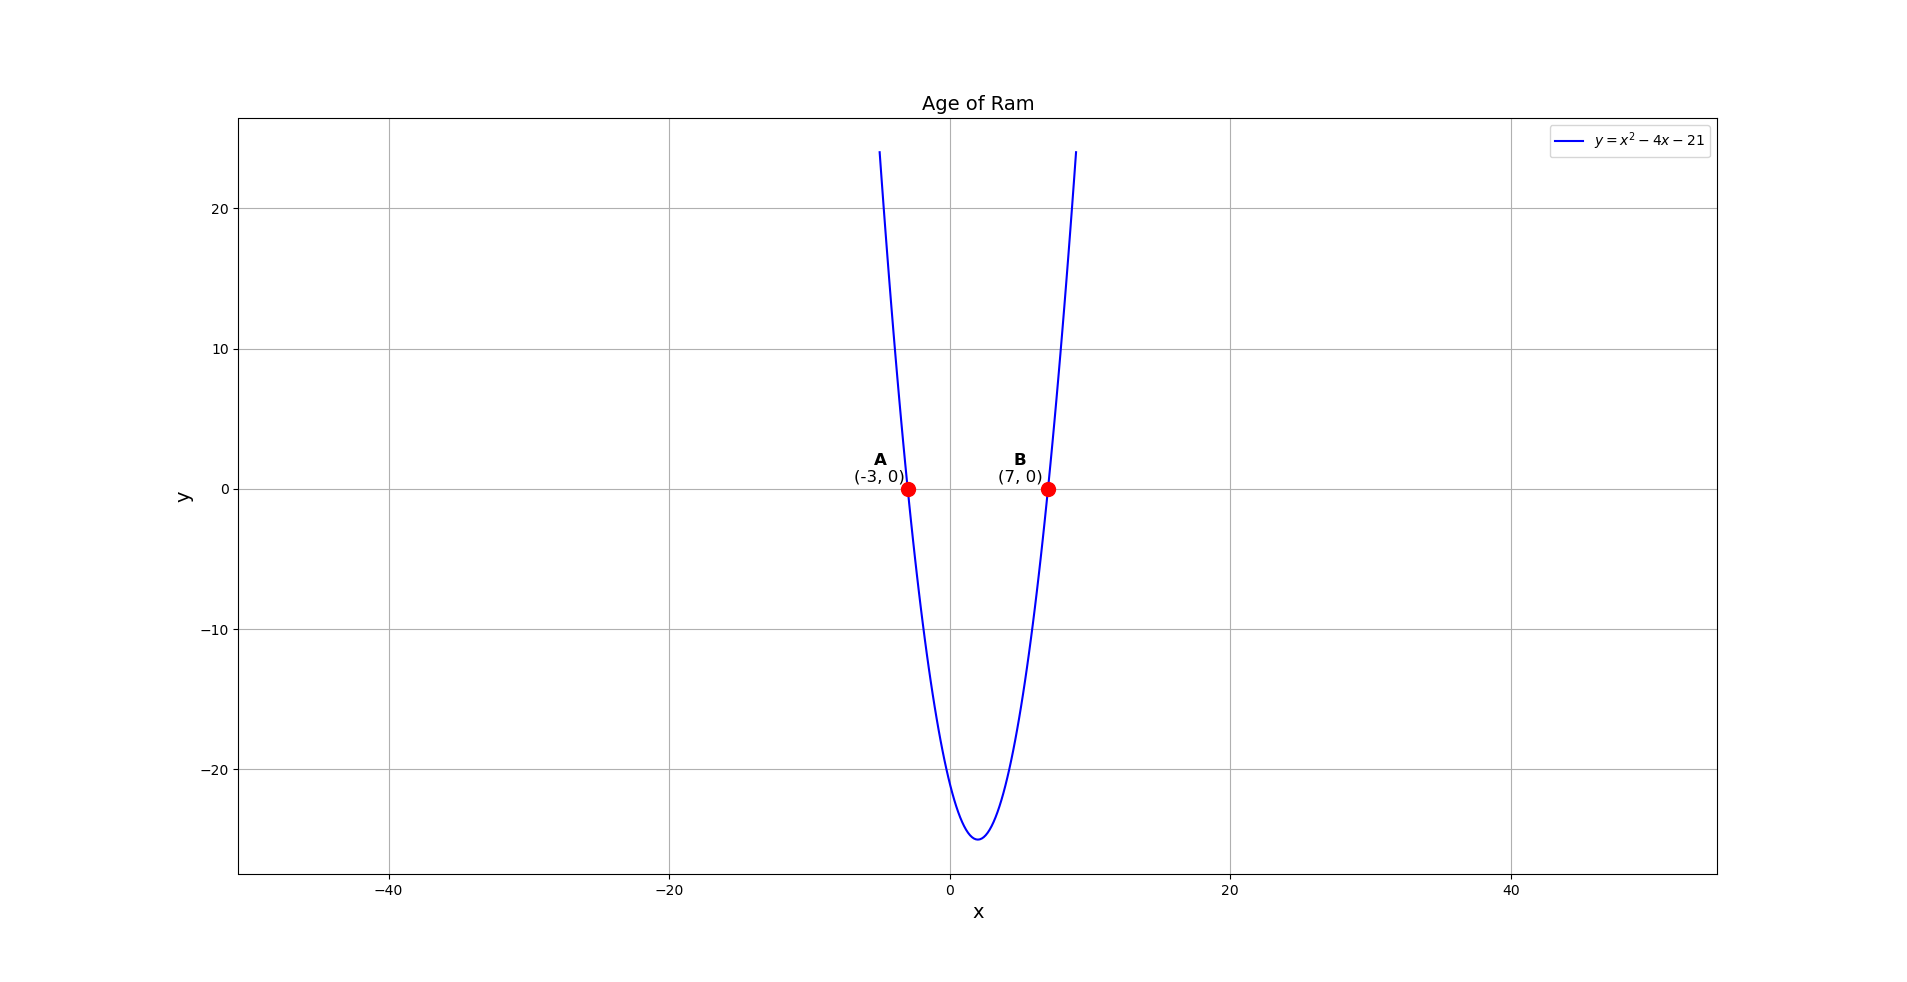
\includegraphics[width=0.9\columnwidth]{figs/fig1.png}
	\caption{}
   \label{}
\end{figure}
\end{document}
